%%%%%%%%%%%%%%%%%%%%%%%%%%%%%%%%%%%%%%%%%%%%%%%%%%%%%%%%%%%%%%%%%%%%%%%%%%%%%%%%%%%%%%%%%%%%%%%%%%%%

\documentclass[a4,12pt]{article}

%%%%%%%%%%%%%%%%%%%%%%%%%%%%%%%%%%%%%%%%%%%%%%%%%%%%%%%%%%%%%%%%%%%%%%%%%%%%%%%%%%%%%%%%%%%%%%%%%%%%

% \usepackage{aeguill}
\usepackage[utf8]{inputenc}
\usepackage{eurosym}
\usepackage[hmargin=1cm, vmargin=1.5cm, noheadfoot, a4paper]{geometry}
\usepackage{tikz}
\usetikzlibrary{calc}

%%%%%%%%%%%%%%%%%%%%%%%%%%%%%%%%%%%%%%%%%%%%%%%%%%%%%%%%%%%%%%%%%%%%%%%%%%%%%%%%%%%%%%%%%%%%%%%%%%%%

\def\og~{{\fontencoding{T1}\selectfont%
	   \guillemotleft}}
\def\fg\ {\unskip{\fontencoding{T1}\selectfont%
	   \guillemotright}\space}

\def\fpg{\fg \unskip}

%%%%%%%%%%%%%%%%%%%%%%%%%%%%%%%%%%%%%%%%%%%%%%%%%%%%%%%%%%%%%%%%%%%%%%%%%%%%%%%%%%%%%%%%%%%%%%%%%%%%

\pagestyle{empty}

%%%%%%%%%%%%%%%%%%%%%%%%%%%%%%%%%%%%%%%%%%%%%%%%%%%%%%%%%%%%%%%%%%%%%%%%%%%%%%%%%%%%%%%%%%%%%%%%%%%%

\def\width{11mm}
\def\height{13mm}

%%%%%%%%%%%%%%%%%%%%%%%%%%%%%%%%%%%%%%%%%%%%%%%%%%%%%%%%%%%%%%%%%%%%%%%%%%%%%%%%%%%%%%%%%%%%%%%%%%%%

\newcommand{\myfont}[1]{\texttt{\large{#1}}}

\newcommand{\key}[6]{%
  \node (a) at ($ (#1*\width,#2*\height) $) {};
  \draw[gray!50, very thin] %
  ($ (a) $) -- ++(\width,0mm) -- ++(0mm,\height) -- ++(-\width,0mm) -- cycle;
  \draw[black] ($ (a) + (1/3*\width-.5mm,1/3*\height-.5mm) $) node {\myfont{#3}};
  \draw[black] ($ (a) + (1/3*\width-.5mm,2/3*\height+.5mm) $) node {\myfont{#4}};
  \draw[black] ($ (a) + (2/3*\width+.5mm,1/3*\height-.5mm) $) node {\myfont{#5}};
  \draw[black] ($ (a) + (2/3*\width+.5mm,2/3*\height+.5mm) $) node {\myfont{#6}};
}

\newcommand{\skey}[4]{%
  \node (a) at ($ (#1*\width,#2*\height) $) {};
  \draw[gray!50, very thin] %
  ($ (a) $) -- ++(\width,0mm) -- ++(0mm,\height) -- ++(-\width,0mm) -- cycle;
  \draw[black] ($ (a) + (1/3*\width-.5mm,1/2*\height) $) node {\myfont{#3}};
  \draw[black] ($ (a) + (2/3*\width+.5mm,1/2*\height) $) node {\myfont{#4}};
}

\newcommand{\ckey}[3]{%
  \node (a) at ($ (#1*\width,#2*\height) $) {};
  \draw[gray!50, very thin] %
  ($ (a) $) -- ++(\width,0mm) -- ++(0mm,\height) -- ++(-\width,0mm) -- cycle;
  \draw[black] ($ (a) + (1/2*\width,1/2*\height) $) node {\myfont{#3}};
}

\newcommand{\ctwokey}[4]{%
  \node (a) at ($ (#1*\width,#2*\height) $) {};
  \draw[gray!50, very thin] %
  ($ (a) $) -- ++(\width,0mm) -- ++(0mm,\height) -- ++(-\width,0mm) -- cycle;
  \draw[black] ($ (a) + (1/2*\width,1/3*\height) $) node {\myfont{#3}};
  \draw[black] ($ (a) + (1/2*\width,2/3*\height) $) node {\myfont{#4}};
}

\begin{document}
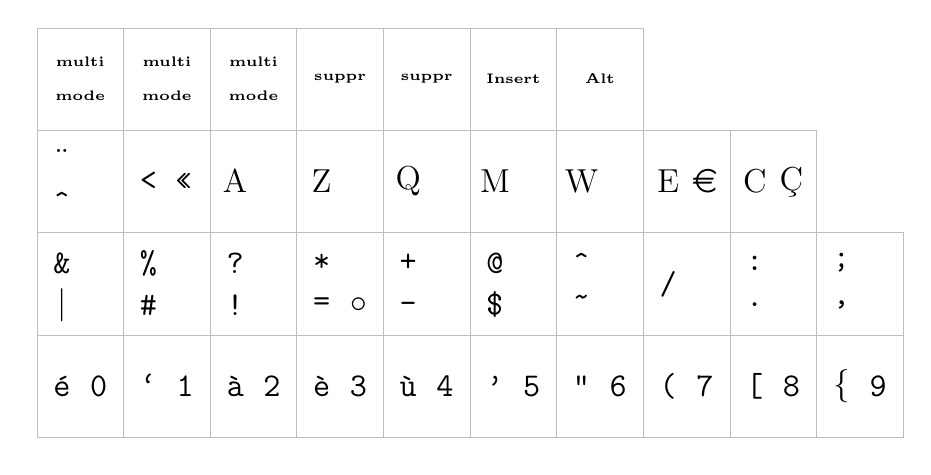
\begin{tikzpicture}
  \skey{0}{0}{é}{0}
  \skey{1}{0}{`}{1}
  \skey{2}{0}{à}{2}
  \skey{3}{0}{è}{3}
  \skey{4}{0}{ù}{4}
  \skey{5}{0}{'}{5}
  \skey{6}{0}{"}{6}
  \skey{7}{0}{(}{7}
  \skey{8}{0}{[}{8}
  \skey{9}{0}{\{}{9}
  %
  \key{0}{1}{\textbar}{\&}{}{}
  \key{1}{1}{\#}{\%}{}{}
  \key{2}{1}{!}{?}{}{}
  \key{3}{1}{=}{*}{$\circ$}{}
  \key{4}{1}{-}{+}{}{}
  \key{5}{1}{\$}{@}{}{}
  \key{6}{1}{\textasciitilde}{\textasciicircum}{}{}
  \skey{7}{1}{/}{}
  \key{8}{1}{.}{:}{}{}
  \key{9}{1}{,}{;}{}{}
  %
 \key{0}{2}{\textasciicircum}{$\ddot{}$}{}{}
 \skey{1}{2}{<}{{\fontencoding{T1}\selectfont\guillemotleft}}
 \renewcommand{\myfont}[1]{\large{#1}}
 \skey{2}{2}{A}{}
 \skey{3}{2}{Z}{}
 \skey{4}{2}{Q}{}
 \skey{5}{2}{M}{}
 \skey{6}{2}{W}{}
 \skey{7}{2}{E}{\euro}
 \skey{8}{2}{C}{Ç}
 %
 \renewcommand{\myfont}[1]{\textbf{\tiny{#1}}}
 \ctwokey{0}{3}{mode}{multi}
 \ctwokey{1}{3}{mode}{multi}
 \ctwokey{2}{3}{mode}{multi}
 \ckey{3}{3}{suppr}
 \ckey{4}{3}{suppr}
 \ckey{5}{3}{Insert}
 \ckey{6}{3}{Alt}
\end{tikzpicture}

\end{document}

%%%%%%%%%%%%%%%%%%%%%%%%%%%%%%%%%%%%%%%%%%%%%%%%%%%%%%%%%%%%%%%%%%%%%%%%%%%%%%%%%%%%%%%%%%%%%%%%%%%%
%%% Local Variables: 
%%% mode: latex
%%% TeX-master: t
%%% End: 
%%%%%%%%%%%%%%%%%%%%%%%%%%%%%%%%%%%%%%%%%%%%%%%%%%%%%%%%%%%%%%%%%%%%%%%%%%%%%%%%%%%%%%%%%%%%%%%%%%%%
